\chapter{数値実験}

本章では,提案したアルゴリズムの有効性を検証するための実験を行う.

\section{基本実験}

人工ネットワーク

また,比較のため,アルゴリズムに示したBrandesのアルゴリズムの結果と比較する.

図\ref{fig:exp-insert-node}は挿入時の頂点数に対する実行時間を比較したものである.平均次数は$10$で固定している.

\begin{figure}[tb]
  \centering
  \includegraphics[width=\linewidth]{exp-insert-node.pdf}
  \caption{挿入時の頂点数に対する実行時間の比較}
  \label{fig:exp-insert-node}
\end{figure}

図\ref{fig:exp-insert-ratio}は挿入時の頂点数と平均次数に対する,2手法の実行時間の比である.

\begin{figure}[tb]
  \centering
  \includegraphics[width=\linewidth]{exp-insert-ratio.pdf}
  \caption{挿入時の頂点数と平均次数に対する実行時間の比}
  \label{fig:exp-insert-ratio}
\end{figure}

図\ref{fig:exp-insert-recalc}は挿入時に距離を更新した頂点の割合に対する実行時間を表したものである.

\begin{figure}[tb]
  \centering
  \includegraphics[width=\linewidth]{exp-insert-recalc.pdf}
  \caption{挿入時に距離を更新した頂点の割合に対する実行時間}
  \label{fig:exp-insert-recalc}
\end{figure}

\begin{figure}[tb]
  \centering
  \includegraphics[width=\linewidth]{exp-delete-node.pdf}
  \caption{挿入時の頂点数に対する実行時間の比較}
  \label{fig:exp-delete-node}
\end{figure}

\begin{figure}[tb]
  \centering
  \includegraphics[width=\linewidth]{exp-delete-ratio.pdf}
  \caption{挿入時の頂点数と平均次数に対する実行時間の比}
  \label{fig:exp-delete-ratio}
\end{figure}

\begin{figure}[tb]
  \centering
  \includegraphics[width=\linewidth]{exp-delete-recalc.pdf}
  \caption{挿入時に距離を更新した頂点の割合に対する実行時間}
  \label{fig:exp-delete-recalc}
\end{figure}

\section{実データに対する実験}

ネットワークは2270頂点,2663辺を有する.
ネットワークの図を図\ref{fig:net-ou1}に示す.

\begin{figure}[tb]
  \centering
  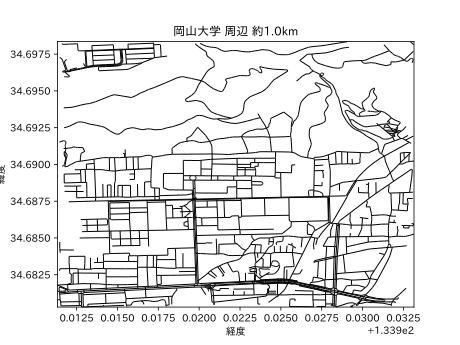
\includegraphics[width=.5\textwidth]{road-ou1.pdf}
  \caption{実験で用いるネットワーク}
\end{figure}

\begin{table}[tb]
  \centering
  \caption{実データに対する挿入時の実験結果}
  \begin{tabular}{lr}
    \hline
    計算方法 & 平均実行時間[s] \\ \hline
    再計算 & 0.370 \\ \hline
    更新 & 0.748 \\ \hline\hline
    再計算した頂点の割合 & 0.995 \\ \hline
  \end{tabular}
\end{table}

\begin{table}[tb]
  \centering
  \caption{実データに対する削除時の実験結果}
  \begin{tabular}{lr}
    \hline
    計算方法 & 平均実行時間[s] \\ \hline
    再計算 & 0.379 \\ \hline
    更新 & 34.576 \\ \hline\hline
    再計算した頂点の割合 & 1.000 \\ \hline
  \end{tabular}
\end{table}
